\providecommand{\muh}{\hat{\mu}}
\providecommand{\yh}{\hat{y}}

\chapter{\label{chap:intro} Introduction}

% Motivation.1: information summarization.
One of the most exciting applications of natural language processing ahead of us is the development of systems that will help us digest the vast amount information being generated around the world.
For example, we will one day be able to rely on 
text summarization (TS) systems to condense the most salient information from one or more related articles into as few words as necessary (\reffig{intro:overview}(a)).
We will be be able to get targeted summaries through open-ended question answering systems (OQA) (\reffig{intro:overview}(b)).
Finally, knowledge base population (KBP) systems  will be able to read large document troves (or the Internet) and present succinct, structured, summaries about the people and organizations mentioned within (\reffig{intro:overview}(c)).

\begin{figure}[!p]
  \centering
  \begin{subfigure}[b]{.42\textwidth}
    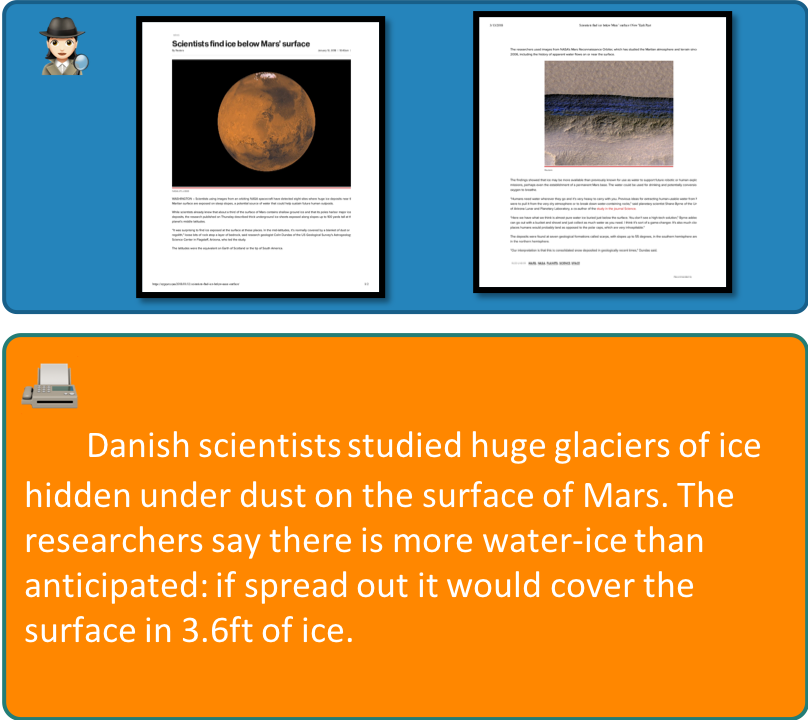
\includegraphics[width=\textwidth]{figures/task_ts}
    \caption{Text summarization}
  \end{subfigure}

  \begin{subfigure}[b]{.42\textwidth}
    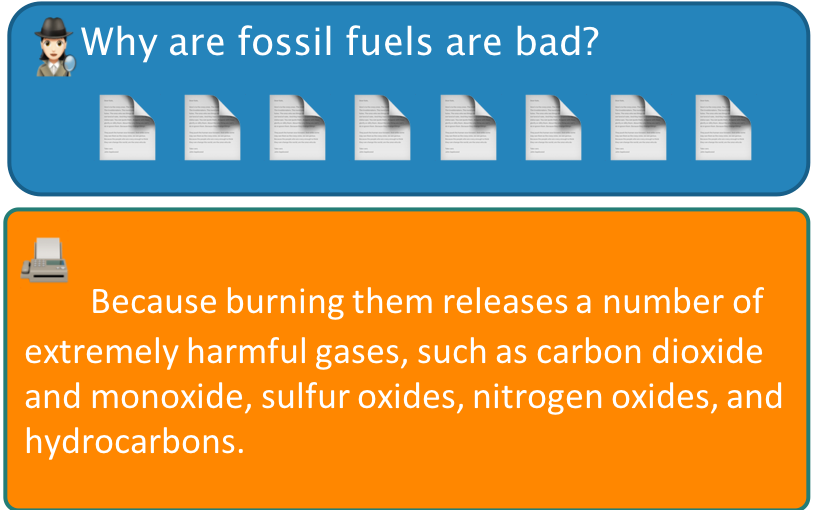
\includegraphics[width=\textwidth]{figures/task_oqa}
    \caption{Open question answering}
  \end{subfigure}

  \begin{subfigure}[b]{.42\textwidth}
    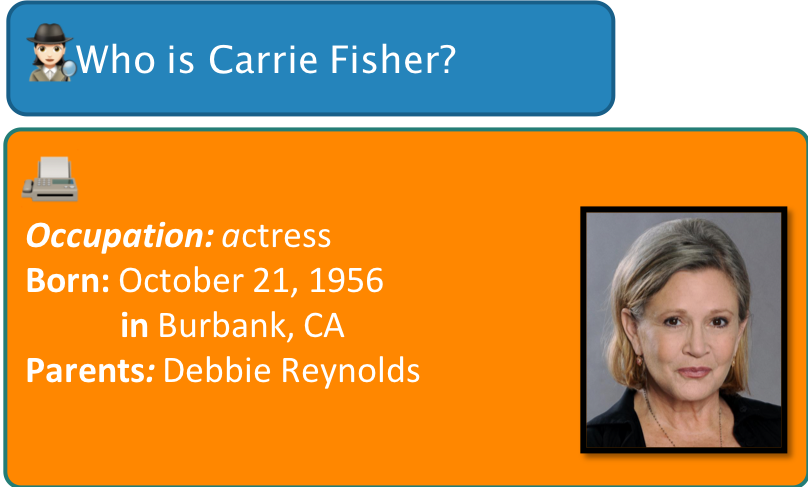
\includegraphics[width=\textwidth]{figures/task_kbp}
    \caption{Knowledge base population}
  \end{subfigure}

  \caption[Overview of some information summarization tasks]{\label{fig:intro:overview} An overview of some information summarization tasks, listed in increasing specificity:
  (a) Text summarization: seeks to identify the most salient information contained within one (or more) article(s) and describe this information in as few words as necessary.
  (b) Open-response question answering: provides very-targeted summaries that address a specific question.
  (c) Knowledge base population: reads documents from a large corpus and generates linked entity-centric summaries for every person and organization mentioned within.
  }
\end{figure}

% Motivation.2: A brief history of work in the area
Indeed, this broad vision of what we call \textit{information summarization} has been the goal of many natural language processing systems dating as far back as the 1950s~\citep{luhn1958automatic}.
Research has shown that having access to document summaries significantly improves user satisfaction and their ability to complete fact-gathering tasks~\citep{mani1999tipster, mckeown2005summaries}. 
Building these systems, however, remains a challenge.
Today, we are seeing a resurgence in interest in information summarization systems, with over 150 papers published at top NLP conferences in just the last year (2017--18).\footnote{%
This number was estimated by looking at papers with topics pertaining to information extraction, question answering and text summarization systems.} 


% Motivation.3: Measurement is broken
Despite years of effort, it is unclear whether we are actually making forward progress on these tasks.
Take the task of text summarization for example:
\citet{brandow1995automatic} conducted a large scale human evaluation of different text summarization systems and found that the baseline of simply taking the lead-paragraph significantly outperformed automatic systems. 
Ten years later, \citet{passonneau2005applying} report that half of the systems participating in the DUC-2005 text summarization challenge did worse than the baseline.
Even today, we find that recent ``state-of-the-art'' neural network based text summarization systems fare poorly on human evaluations of language quality relative to simpler extractive systems.
The performance of knowledge base population systems as tracked by the TAC KBP challenge has been similarly halting.
While there are many reasons for this slow progress, we believe that the lack of an effective evaluation methodology remains one of the most important ones.
%\pl{now this is about text summarization specifically, but do you want to talk more broadly?  for example, you could even bring in MT}

% Our contribution.
The ultimate goal of this thesis is to enable the development of better information summarization systems by addressing systemic problems in how we evaluate them.
In this work, we attribute the inherent \textit{incompleteness} of existing evaluation datasets as the key bottleneck to reliably measuring the performance of information summarization systems.
We posit that collecting on-demand human feedback is necessary to economically obtaining meaningful measures of system quality by resolving this incompleteness.
Our key technical contribution is applying techniques from statistical estimation to reliably integrate human feedback in a cost-effective manner.

\begin{figure}
  \hfill
  \begin{subfigure}{0.45\textwidth}
  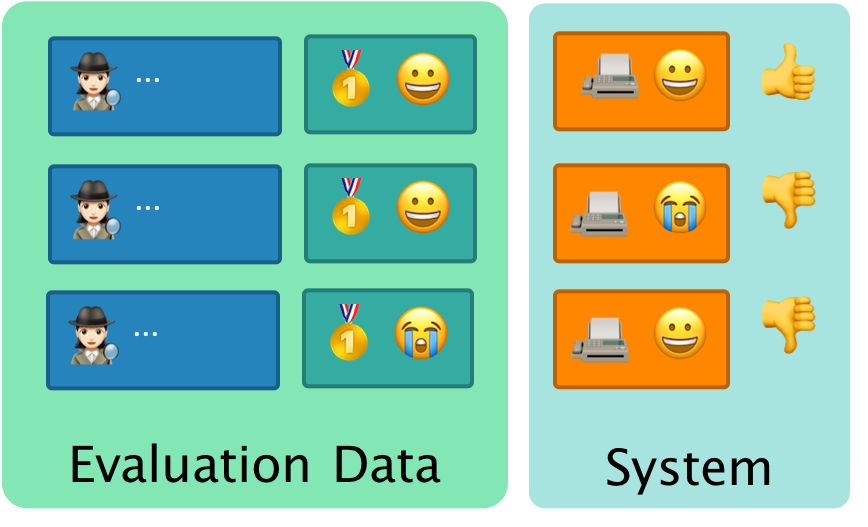
\includegraphics[width=\textwidth]{figures/classification}
  \caption{Classification}
  \end{subfigure} 
  \hfill
  \begin{subfigure}{0.45\textwidth}
  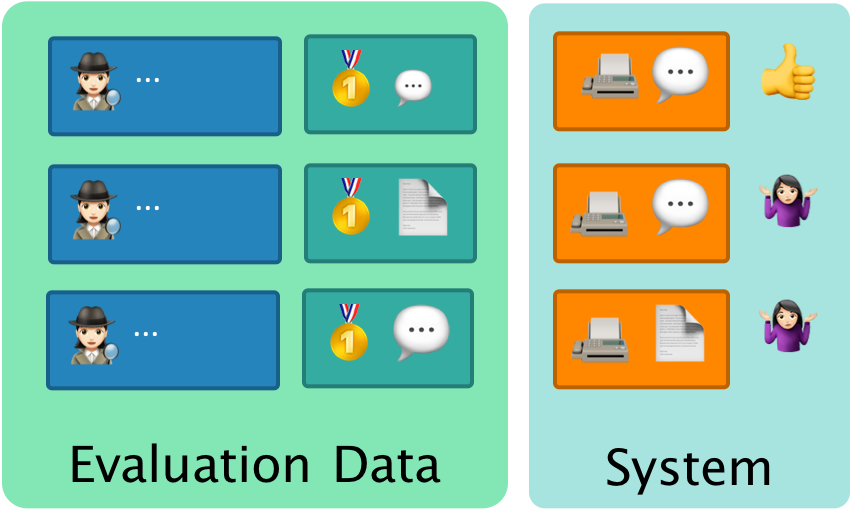
\includegraphics[width=\textwidth]{figures/generation}
  \caption{Open-response}
  \end{subfigure}
  \hfill

  \caption[Complete and incomplete evaluation sets]{\label{fig:intro:evaluation-data} 
  Much of our evaluation methodology relies on an evaluation dataset that contains paired inputs (represented by blue boxes) and outputs (green boxes).
  (a) When the outputs belong to a closed class, e.g.\ in sentiment classification, it is easy to compare the output of a system (orange boxes) with the reference answer and hence evaluate its performance.
  (b) On the other hand, in the information summarization tasks we are interested in, there are many possible correct answers. As a result, a system that produces a response that does not match the reference answer is not necessarily incorrect; we simply don't know how to evaluate it. In this sense, the evaluation data is \textit{incomplete}.
  }
\end{figure}
\section{The incompleteness of static evaluation sets}
At its core, the prevalent evaluation methodology for most tasks in natural language processing, including the aforementioned information summarization tasks, relies on a evaluation dataset that contains pairs of query inputs and expected outputs (\reffig{evaluation-data}).
On classification problems, e.g.\ sentiment classification or topic identification, the output typically belongs to a small closed class (e.g.\ positive, neutral or negative sentiment).
When a system also predicts an output belonging to this closed class, we know whether or not it made a mistake by comparing if its prediction is the same as the expected class; 
Thus, in these settings, we can measure the quality of different systems on the classification task by simply collecting a sufficiently large evaluation dataset.\footnote{%
Of course, care must be taken to ensure the evaluation dataset collected is reflective of the end-goal for the task.}

Unfortunately, in the information summarization tasks we've seen above, the desired output is not simply a class label but rather an arbitrary piece of text (e.g.\ in TS and OQA) or an arbitrarily large collection of facts (e.g.\ for KBP).
The assumption that there exists a unique knowable correct output simply does not hold.
In this sense, the static evaluation dataset we discussed earlier \textit{can not} contain every possible correct answer and as a result is \textit{incomplete}.
Let's look at some examples of how incompleteness manifests in practice and what its consequences on evaluation could be.

\begin{figure}
  \hfill
  \begin{subfigure}[t]{0.45\textwidth}
    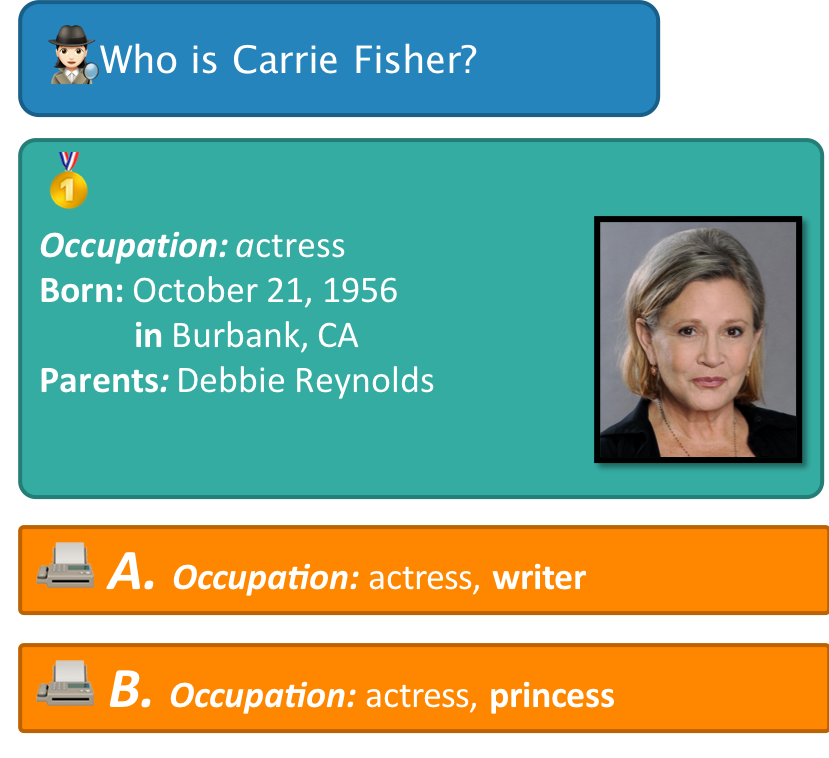
\includegraphics[width=\textwidth]{figures/err-kbp}
    \caption{\label{fig:intro:example-kbp} Knowledge base population.}
  \end{subfigure}
  \hfill
  \begin{subfigure}[t]{0.45\textwidth}%
    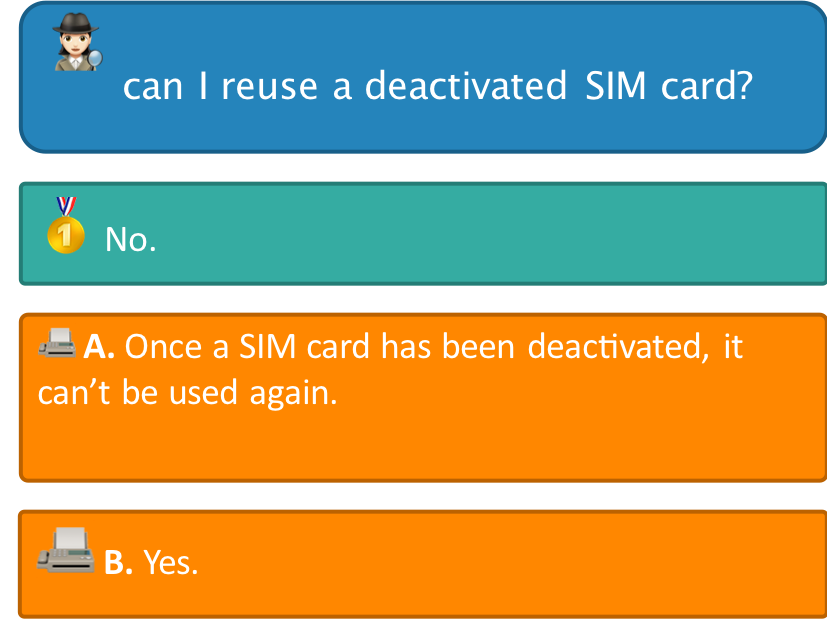
\includegraphics[width=\textwidth]{figures/err-oqa}
    \caption{\label{fig:intro:example-qa} Open-response question answering.}
  \end{subfigure}
  \hfill

  \hfill
  \begin{subfigure}[t]{0.95\textwidth}
    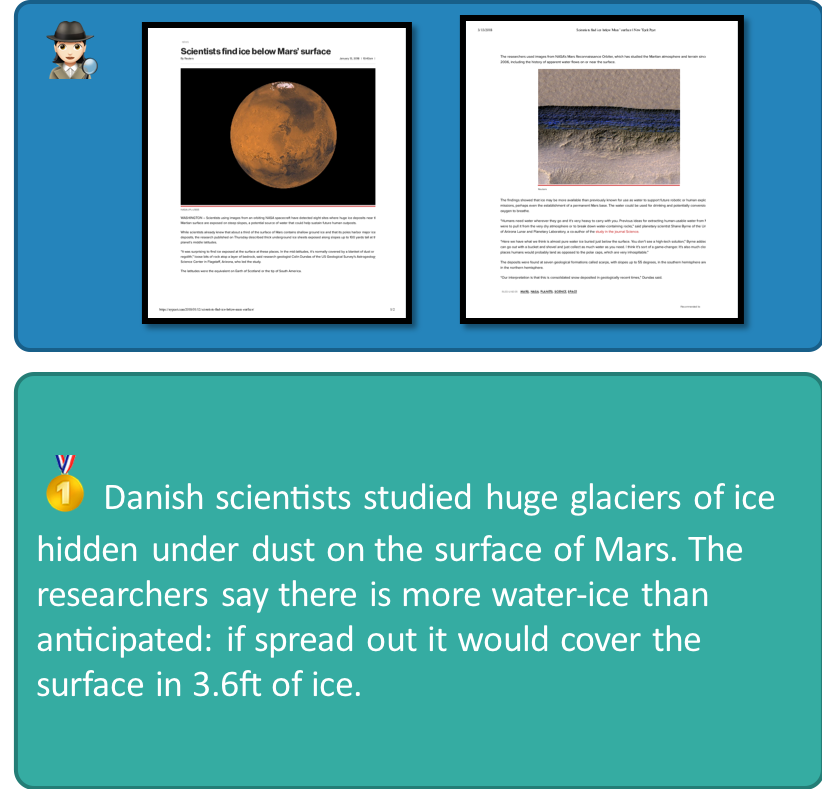
\includegraphics[width=0.45\textwidth]{figures/err-summ1}
    \hfill
    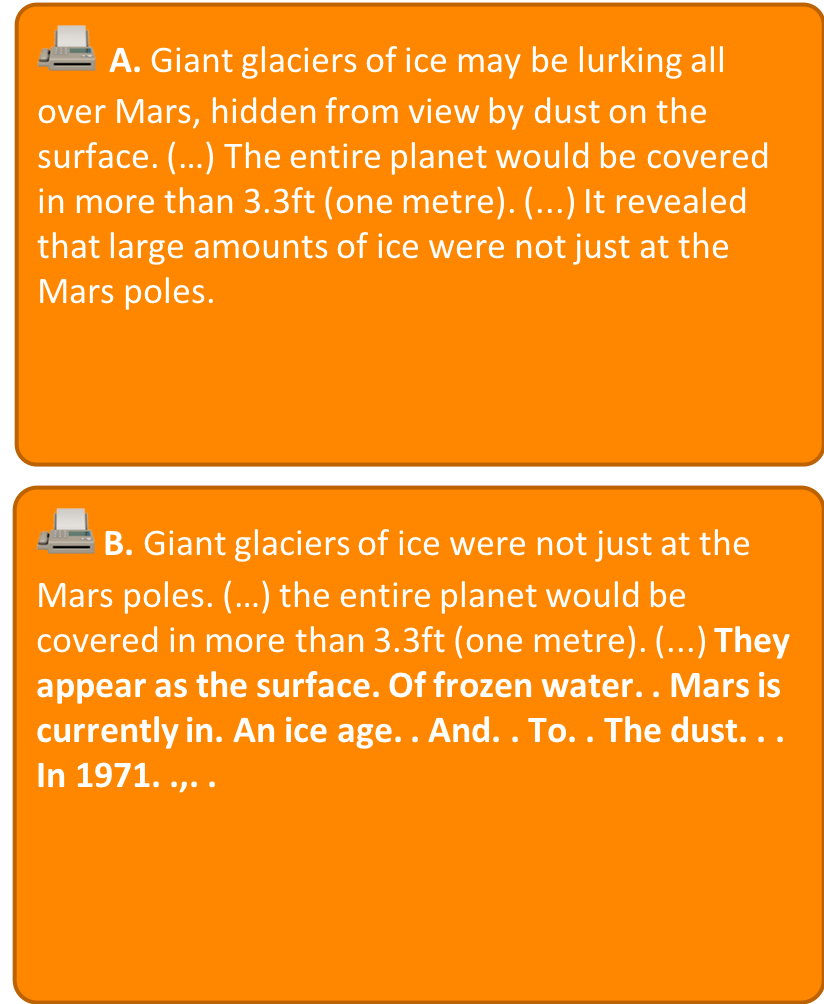
\includegraphics[width=0.45\textwidth]{figures/err-summ2}
    \caption{\label{fig:intro:example-summarization} Text summarization. }
  \end{subfigure}
  \hfill

  \caption[Examples highlighting the limitations of incomplete evaluation sets]{\label{fig:intro:examples} Examples where the reference data is unable to evaluate a system's response:
  (a) Knowledge base population: here, the incomplete reference data is unable to identify that it is a true that Carrie Fisher was also an author, but not that she is a `princess'.
  (b) Open-response question answering: it is common for systems to output a paraphrase of the reference answer and thus to be judged incorrect despite reporting the right answer.
  (c) Text summarization: systems rarely produce output that is identical to the reference answer and word-overlap based similarity measures often prefer bad responses with high lexical similarity over good responses that more more lexically distinct.  
  }
\end{figure}

%\paragraph{Knowledge base Population.}
\reffig{intro:example-kbp} shows the candidate output of two KBP systems for Carrie Fisher, the late actress who played Princess Leia in the Star Wars movie franchise.
The incomplete KBP reference data only specifies that Ms.\ Fisher is an actress and thus the evaluation is unable to judge whether the system that identifies her to also be an author (which is correct) is better or worse than one that identifies her to also be a princess (which is incorrect): by default, the evaluation penalizes both decisions equally.
As a consequence, using this evaluation as an empirical guide leads researchers to avoid improvements that would identify Ms.\ Fisher as an actress.
In \refsec{kbpo:analysis} we'll empirically estimate the bias caused by this incompleteness and show that it is often larger than most model improvements.

%\paragraph{Question answering.}
Next, consider an example in question answering:
  here, the fundamental problem is that there are many ways to express the same answer (\reffig{intro:example-qa}).
It is not yet easy to automatically identify whether two phrases mean the same thing and hence fairly judge the output systems produce.
More subtly, we show that this evaluation is biased towards easier questions with short answers that are more likely to be reproduced by a system:
  model improvements that improve answers for harder questions will be ignored by the evaluation.

%\paragraph{Text summarization.}
Finally, consider the evaluation of text summarization systems: a system-generated summary will never exactly match the one in the evaluation dataset.
A common practice in the community is to use a word-overlap based similarity score such as BLEU~\citep{papineni02bleu} or ROUGE~\citep{lin2004rouge}\@.
Unfortunately, these automatic metrics have been shown to correlate extremely poorly with human judgment~\citep{novikova2017why}.
\reffig{intro:example-summarization} shows an example of a published system that learns to game this metric by appending seemingly random words at the end of a summary.
% \pl{Biggest comment: 'summarization' is used kind of used in two ways, and the text kind of vaciliates between text summarization and the larger goal; I think you should focus on the larger goal because the thesis is about more than just text summarization }

\section{Addressing incompleteness with human feedback}
We've just seen how the incompleteness of our evaluation sets can introduce bias.
How fundamental is incompleteness?
Broadly, we consider two ends of the spectrum: when the incompleteness is large but ``finite'' and when the incompleteness is truly ``infinite''.

In the finite setting, it is possible, though perhaps not economical, to exhaustively annotate the output space.
Consider knowledge base population as an example: here it is possible to minimize the impact of incompleteness by exhaustively annotating a sufficiently large document collection of about 100,000 documents, an effort that we estimate would cost at least \$1 million.
Of course, any adjustment in the task definition (e.g.\ the relation schema) would require a fresh batch of annotations.
In this sense, handling finite incompleteness can be viewed as a prudent cost-saving measure.
On the other hand, the number of correct wordings for an answer in text summarization or open-ended question answering are nearly endless; we doubt that any size of static datasets would be sufficient to ameliorate the problem here.
We consider the incompleteness in such settings to be infinite. 

The crux of the problem is estimating the impact of instances that are unknown to the automatic evaluation that relies on a static dataset.
We exploit the fact that the answers to these instances are obvious to humans and propose asking people for feedback \textit{on-demand} using advances in crowdsourcing.
In this work, we advocate moving from annotating data in batches to annotating data \textit{on-demand}.

Apart from fixing the problem of incompleteness, incorporating human feedback has several ancillary benefits.
First, it ensures that our evaluation does not diverge from the end goals of the task.
Second, it provides \textit{qualitative} guidance to help us identify opportunities for improvements.
%As an example of this latter point, in \refchap{kbpo} we show how combining human labels with statistical estimators can be used to conduct fine-grained error analysis for KBP, and in \refchap{price} we show how collecting human edits as feedback can be used for error analysis in text generation.

%Finally, the role of evaluation is two-fold: first to provide \textit{quantitative} guidance that help us empirically validate improvements to systems, and secondly \textit{qualitative} guidance to help us identify opportunities for improvements.

\section{Integrating human feedback with statistical estimators}
While human evaluation is often regarded as a gold standard for evaluation, it is also considered to be too expensive to be used as when iterating on models.
The key question this thesis tries to answer then is: can we reduce the cost of human annotation in evaluation while maintaining its fidelity?
Our core contribution is in addressing the problem of incompleteness for two extremes: problems where incompleteness is large but finite (KBP), and problems where incompleteness is truly infinite (text summarization and open-response question answering).
In both settings, we hold \textit{unbiased} estimation as our bar: the methods we describe are guaranteed to produce the same results that an exhaustive human evaluation would have.

\paragraph{Amortizing costs when incompleteness is finite.}
In settings where incompleteness is finite, it is likely that two different systems produce an overlapping set of outputs, suggesting that we may can leverage human annotations obtained for one system to evaluate another.
The key challenge is guarding against what we call representation bias: we don't want to skew the evaluation towards a particular class of systems simply because our evaluation data came from these systems.
We tackle this problem in \refchap{kbpo} using a novel importance-reweighted estimator. We apply the estimator to evaluate KBP systems and show that we are able to reduce the cost of obtaining human annotations by a factor of 4.

\paragraph{Finding limitations when incompleteness is infinite.}
On the other end of the spectrum, in tasks like text summarization or open-ended question answering, the output produced consists of free form text: it  is extremely unlikely that two systems will ever agree on the output they produce.
Here, it seems natural to rely on some ``similarity'' measure that may allow us to match two similar, but non-identical responses.
In \refchap{price}, we derive an optimal estimator to combine such a similarity metric with human feedback based on control variates~\citep{owen2013monte}.
Our theoretical analysis allows us to characterize when it is possible to reduce human annotation costs while guaranteeing unbiasedness.
We show that for both text summarization and open-ended question answering current cost savings are modest, about 10--15\%, owing to both the poor quality of existing automatic metrics and the inherent annotator variance for these subjective tasks.

\paragraph{Beyond evaluation.}
Thus far, we have focused on the use of human feedback during evaluation and not on how that evaluation can be used to improve the original system.
We turn to this problem in the \refchap{otj}, where we show how human feedback can be effectively integrated \textit{at test-time} to continuously improve on the performance of the original system.
We call this setting  ``on-the-job learning'' because our model learns as inputs arrive: we use real-time crowdsourcing to resolve uncertainty where needed and output our prediction once the model is confident.
The human feedback is used to train the model and as the model improves over time, the reliance on crowdsourcing queries decreases. 
We cast the problem as a stochastic game and use Bayesian decision theory to balance latency, cost, and accuracy objectives in a principled way. 
Unfortunately, computing the optimal policy is intractable, so we develop an approximation based on Monte Carlo Tree Search.
We tested our approach on three datasets---named-entity recognition, sentiment classification, and image classification.
On the NER task we obtained more than an order of magnitude reduction in cost compared to full human annotation, while boosting performance relative to the expert provided labels.

\section{Thesis outline}
The rest of the thesis is structured as follows:
In \refchap{setup}, we'll cover the necessary statistical prerequisites to understand what bias means and how different evaluation methodologies can be quantitatively compared.
We will also review some background in the different evaluation strategies that have been adopted in natural language processing and the goals that each seeks to meet.
In \refchap{kbpo}, we will study finite incompleteness using knowledge base population as our motivating example.
We'll see how incompleteness can be measured and how we can correct for it by combining on-demand human annotations with a novel statistical estimator.
In \refchap{price}, we move over to study infinite incompleteness using open question answering and text summarization as motivating examples.
We'll see how automatic metrics can be optimally combined with human feedback to reduce the costs of human evaluation.
Unfortunately, we'll show that in practice cost savings are modest: 
However, our optimality result lets us step back and observe that our empirical results actually highlight fundamental limitations in using automatic metrics for unbiased evaluation. 
In \refchap{otj}, we change gears and look at how we can use human feedback while learning: we propose a new learning paradigm, ``on-the-job learning'', that allows the model to query for human feedback when it is not confident in its predictions.
Finally, in \refchap{discussion}, we conclude this thesis with a discussion on the further uses of human feedback in building natural language systems.
Our discussion touches upon possible opportunities to improve upon human evaluation as a methodology for natural language generation tasks and how human feedback provides us with a more holistic view of evaluation.
